\documentclass[12pt, a4paper]{article}

\usepackage{array}
\usepackage[portuguese]{babel}
\usepackage{chngpage}
\usepackage{float}
\usepackage[a4paper, margin=2cm]{geometry}
\usepackage{graphicx}
\usepackage{hyperref}
\usepackage{setspace}
\usepackage{xcolor}

\title{\Huge \textbf{Computação Gráfica \\ \Large Trabalho Prático -- Fase I}}
\date{2 de março 2025}
\author{Grupo \textbf{\color{red} TODO}}

\begin{document}

\begin{center}
    
\includegraphics[width=0.25\textwidth]{res/cover/EE-C.eps}
\end{center}

\chardef\_=`_
\onehalfspacing
\setlength{\parskip}{\baselineskip}
\setlength{\parindent}{0pt}
\def\arraystretch{1.5}

{\let\newpage\relax\maketitle}
\maketitle
\thispagestyle{empty}

\vspace*{\fill}

\begin{adjustwidth}{-2cm}{-2cm} % These values only need to be large enough to center the table
    \begin{center}
        \begin{tabular}{>{\centering}p{0.25\textwidth}
                        >{\centering}p{0.25\textwidth}
                        >{\centering}p{0.25\textwidth}
                        >{\centering\arraybackslash}p{0.25\textwidth}}
            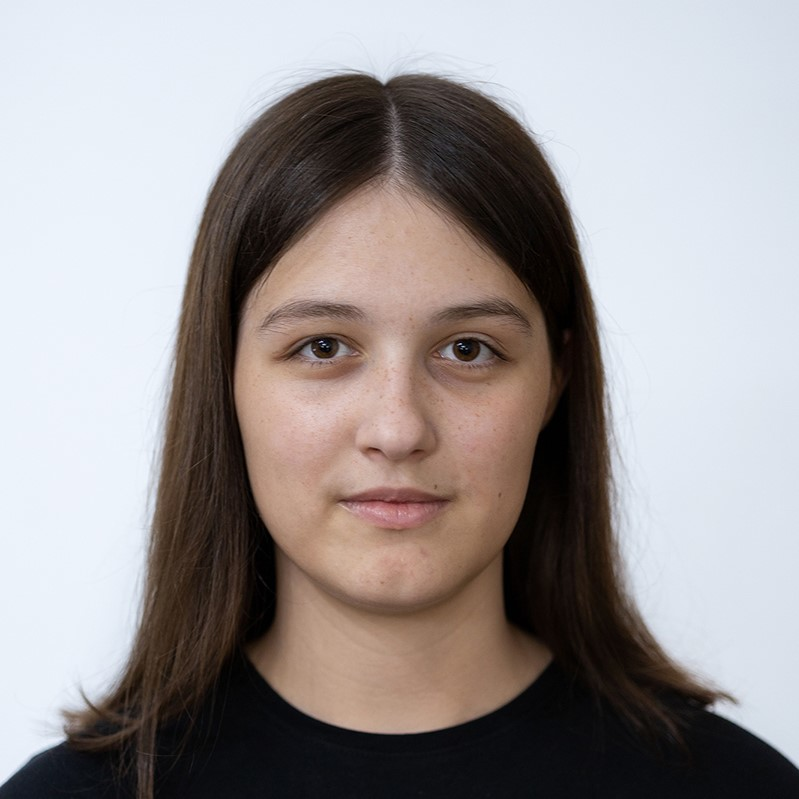
\includegraphics[width=3.5cm]{res/cover/A104437.png} &
            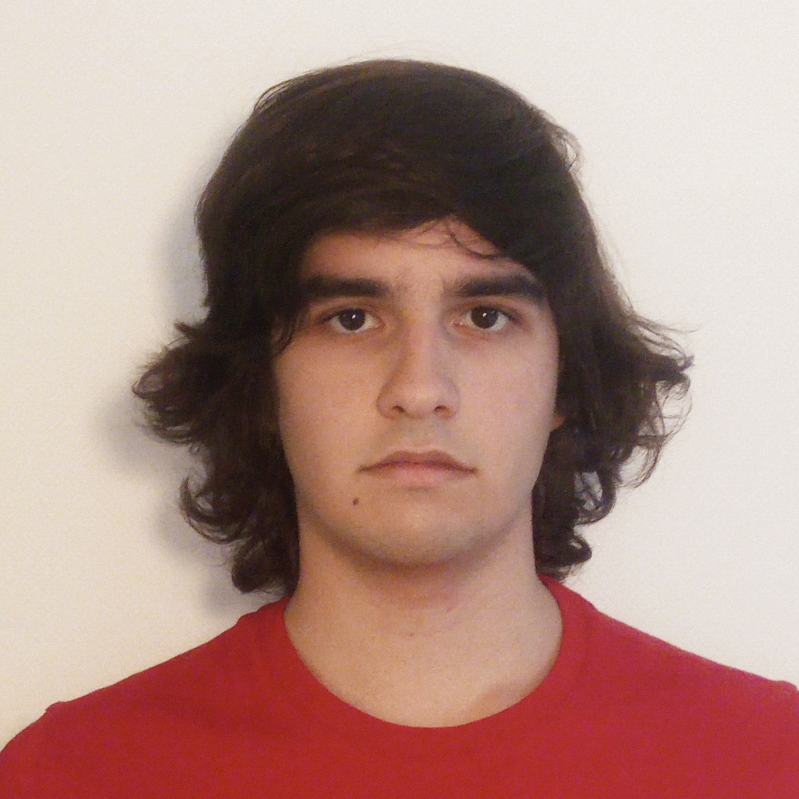
\includegraphics[width=3.5cm]{res/cover/A104348.png} &
            
\includegraphics[width=3.5cm]{res/cover/A90817.png} &
            
\includegraphics[width=3.5cm]{res/cover/A104179.png} \\

            Ana Oliveira & Humberto Gomes & Mariana Cristino & Sara Lopes \\
            A104437      & A104348        & A90817           & A104179
        \end{tabular}
    \end{center}
\end{adjustwidth}

\pagebreak

\begin{abstract}
    \textbf{\color{red} TODO - resumo}
\end{abstract}

\section{\emph{Generator}}

\textbf{\color{red} TODO - \emph{generator}}

\section{\emph{Engine}}

\textbf{\color{red} TODO - \emph{engine}}

\section{Resultados obtidos}

\textbf{\color{red} TODO - resultados}

\section{Conclusão e Trabalho Futuro}

A primeira fase do projeto foi concluída com sucesso, de modo que os objetivos previamente definidos
foram alcançados. A implementação de Vertex Buffer Objects (VBOs) para a otimização da renderização
representa um avanço significativo na eficiência do engine, permitindo um processamento mais rápido
e eficaz dos dados dos vértices.

Em relação ao trabalho futuro, pretendemos realizar uma reestruturação da organização hierárquica do
mundo. A abordagem inicial, que privilegiava uma estrutura linear, será substituída por um sistema
de grupos que permitirá a aplicação de transformações a conjuntos de modelos de forma simultânea.
Esta alteração, motivada pela análise das fases subsequentes do projeto, possibilitará a gestão
eficiente de objetos relacionados.

Adicionalmente, tencionámos expandir as capacidades da câmara, implementando três modos distintos de
visualização: orbital, livre e em terceira pessoa. Esta diversidade de perspetivas enriquecerá a
experiência do utilizador e permitirá a exploração de diferentes estilos de interação com as cenas
3D.

A implementação das transformações geométricas solicitadas na segunda fase – translação, rotação e
escala – é um objetivo prioritário. Estas funcionalidades são essenciais para uma manipulação
precisa dos objetos na cena.

Acreditámos que estas melhorias e adições consolidarão o engine como uma ferramenta robusta e
versátil para a criação de mundos 3D.

\begingroup
\section{Bibliografia}
\renewcommand{\section}[2]{}

\begin{thebibliography}{9}
    \bibitem{exemplo}
        \href{https://youtu.be/dQw4w9WgXcQ}{Um item de exemplo na bibliografia}
\end{thebibliography}
\endgroup

\end{document}
